\documentclass[oneside,a4paper,14pt]{extarticle}
\usepackage[T1,T2A]{fontenc}
\usepackage[a4paper,top=2cm,bottom=2cm,left=2.5cm,right=1.5cm]{geometry}
\usepackage[utf8]{inputenc}
\usepackage[russian]{babel}
\usepackage{textcomp}
\usepackage{indentfirst}
\usepackage{listings}
\usepackage{xcolor}
\usepackage{float}
\usepackage{enumitem}
\usepackage{graphicx}
\usepackage{wrapfig}
\usepackage{caption}
\usepackage{amsmath}
\usepackage{amsfonts}
\usepackage{amsthm}
\usepackage[all]{xy}
\usepackage[breaklinks]{hyperref}
\usepackage{xurl}
\usepackage{titlesec}
% Настройки заголовков
\titleformat{\section}{\large\bfseries}{\thesection}{1em}{}
\titleformat{\subsection}{\large\bfseries}{\thesubsection}{1em}{}
\titleformat{\subsubsection}{\large\bfseries}{\thesubsubsection}{1em}{}
\renewcommand\baselinestretch{1.33}
\setlength{\parindent}{1.25cm}
% Настройки листингов
\lstset{
	basicstyle=\ttfamily\small,
	numbers=left,
	numberstyle=\tiny\color{gray},
	frame=single,
	breaklines=true,
	showstringspaces=false,
	tabsize=2,
	inputencoding=cp1251,
	extendedchars=true,
}
\lstdefinestyle{jsonstyle}{
	language=json,
	basicstyle=\ttfamily\footnotesize,
	keywordstyle=\color{blue}\bfseries,
	stringstyle=\color{red},
	numbers=left,
	numberstyle=\tiny\color{gray},
	frame=single,
	breaklines=true,
	showstringspaces=false,
	tabsize=2,
	extendedchars=true,
}
\begin{document}
	\newpage\thispagestyle{empty}
	\begin{center}
		МИНИСТЕРСТВО НАУКИ И ВЫСШЕГО ОБРАЗОВАНИЯ\\
		РОССИЙСКОЙ ФЕДЕРАЦИИ\\
		ФЕДЕРАЛЬНОЕ ГОСУДАРСТВЕННОЕ БЮДЖЕТНОЕ\\
		ОБРАЗОВАТЕЛЬНОЕ УЧРЕЖДЕНИЕ ВЫСШЕГО ОБРАЗОВАНИЯ\\
		«ВЯТСКИЙ ГОСУДАРСТВЕННЫЙ УНИВЕРСИТЕТ»\\
		Институт математики и информационных систем\\
		Факультет автоматики и вычислительной техники\\
		Кафедра электронных вычислительных машин
	\end{center}
	\vspace{20mm}
	\begin{center}
		Отчёт по лабораторной работе №5\\
		по дисциплине\\
		<<Промпт-инжиниринг>>\\
		<<Создание и редактирование аудиоконтента с помощью промпт-инжиниринга>>\\
		<<Вариант 29>>\\
	\end{center}
	\vspace{48mm}
	\noindent
	Выполнил студент гр. ИВТб-1303-06-00 \hfill \rule[-0.5mm]{30mm}{0.15mm}\,/Шубин В.Ю./\\[0.5cm]
	Проверил доцент кафедры ЭВМ \hfill \rule[-0.5mm]{30mm}{0.15mm}\,/Колупаев А.В./
	\vfill
	\begin{center}
		Киров\\
		2026
	\end{center}
	\newpage
	\thispagestyle{empty}
	\section*{Введение}
	\noindent\textbf{Цель работы:} Формирование практических навыков построения конвейеров обработки аудиоданных с использованием свободных облачных сервисов и мультимодальных нейронных сетей. Освоение методов параметрической настройки генерации речи, составления текстурных промптов для аудио-сцен и применения контекстной инъекции для точного распознавания зашумлённой речи.
	
	\noindent\textbf{Языковые модели, используемые в работе:}
	\begin{itemize}
		\item \textbf{Zvukogram} \url{https://zvukogram.com} -- облачный сервис синтеза речи с параметрическим управлением (скорость, высота тона)
		\item \textbf{EzAudio} на Hugging Face Space -- модель генерации звуковых эффектов по текстовому описанию
		\item \textbf{Qwen} \url{chat.qwen.ai}
	\end{itemize}
	
	\noindent\textbf{Предметная область варианта 29:} Розыгрыш
	\begin{itemize}
		\item \textbf{Роль А (Шутник):} Сдерживаемый смех, игривый тон. Характер: попытка сохранить серьёзность, хихиканье, переходящее в открытый смех.
		\item \textbf{Роль Б (Жертва):} Раздражение, гнев. Характер: подозрительность, быстрая реакция, переход на крик.
		\item \textbf{Фоновая сцена:} Домашняя обстановка: приглушённый звук телевизора или радио на заднем плане, комнатное эхо.
	\end{itemize}
	\newpage
	\section{Задание №1: Управляемая генерация речи по заданному тексту и параметрам}
	\subsection{Постановка задачи варианта}
	\noindent\textbf{Вариант №29: Розыгрыш}
	\noindent Вам предстоит выступить в роли инженера по синтезу речи, создающего озвучку для телефонного диалога между шутником и жертвой розыгрыша. Ваша задача — выбрать один из доступных онлайн-инструментов (Zvukogram, Voicebot или Parler-TTS) и сгенерировать аудиофайлы для каждой реплики диалога. Ключевое требование — голос не должен звучать монотонно: необходимо использовать доступные настройки сервиса, чтобы передать характер персонажа (сдерживаемый смех шутника, нарастающую агрессию и крик жертвы).
	
	\subsection{Сценарий диалога (10 реплик)}
	\noindent\textit{(курсивом выделены сложные для распознавания сущности)}
	\begin{itemize}
		\item \textbf{Шутник} (сдерживая смех, серьёзным тоном): \\
		--- Алло, здравствуйте. Это служба доставки \textit{«СкороЗон»}. Ваш заказ \textit{«Квантовый пылесос X-9000»} уже выехал.
		\item \textbf{Жертва} (подозрительно, тихо): \\
		--- Какой пылесос? Я ничего не заказывал. Вы точно не ошиблись номером?
		\item \textbf{Шутник} (пытаясь сохранить интонацию оператора): \\
		--- Нет, ошибка исключена. Адрес: улица \textit{Ленина, дом 42, квартира 7Б}. Оплата при получении: \textit{8500 рублей}.
		\item \textbf{Жертва} (раздраженно, повышая голос): \\
		--- \textit{8500}?! За пылесос? Вы что, издеваетесь? У меня нет таких денег!
		\item \textbf{Шутник} (хихикая, срываясь на шёпот): \\
		--- Это премиум-сегмент. Работает на \textit{термоядерном синтезе}. Кстати, курьер просил передать промокод \textit{«ПЫЛЕСОК2026»}.
		\item \textbf{Жертва} (возмущённо, громко): \\
		--- Хватит нести чушь! Я сейчас вызову полицию! Это мошенничество, статья \textit{159 УК РФ}!
		\item \textbf{Шутник} (почти смеясь, пауза): \\
		--- Ой, простите, коллега... Это проверка связи. Ваш смех записан для \textit{«Календаря добрых дел»}.
		\item \textbf{Жертва} (крик, максимальная громкость): \\
		--- Да как ты смеешь?! Я запомнил твой голос! Ты пожалеешь, я напишу жалобу в \textit{Роскомнадзор}!
		\item \textbf{Шутник} (откровенный смех, расслабленно): \\
		--- Не сердитесь, это же просто розыгрыш от \textit{«Клуба веселых соседей»}. Вам подарок: \textit{скидка 15\%} на пиццу.
		\item \textbf{Жертва} (тяжело дыша, всё ещё злится): \\
		--- Убирайся из моего телефона! И чтоб я больше не слышал этого \textit{радио «Юмор FM»}!
	\end{itemize}
	
	\subsection{Настройки голосовых профилей в Zvukogram}
	\noindent\textbf{Шутник:}
	\begin{itemize}
		\item \textbf{Голос:} «Борис» (мужской, лёгкий средний тембр)
		\item \textbf{Скорость:} +10\% (оживлённый, быстрый темп)
		\item \textbf{Высота тона (Pitch):} +2st (игривый, слегка повышенный)
		\item \textbf{Пунктуация:} многоточия... и скобки () для имитации пауз и сдерживаемого смеха
	\end{itemize}
	\noindent\textbf{Жертва:}
	\begin{itemize}
		\item \textbf{Голос:} «Андрей» (мужской, грубый низкий тембр)
		\item \textbf{Скорость:} -10\% $\rightarrow$ +20\% (постепенное ускорение по мере нарастания злости)
		\item \textbf{Высота тона (Pitch):} -1st (глубокий, угрожающий бас)
		\item \textbf{Пунктуация:} восклицательные знаки! и короткие рубленые фразы для передачи крика
	\end{itemize}
	
	\subsection{Скриншоты настроек}
	\begin{figure}[H]
		\centering
		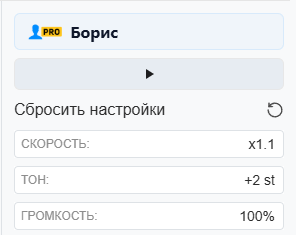
\includegraphics[width=10cm]{1.png}
		\caption{Настройки синтеза речи для роли Шутника}
	\end{figure}
	\begin{figure}[H]
		\centering
		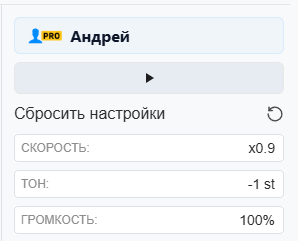
\includegraphics[width=10cm]{2.png}
		\caption{Настройки синтеза речи для роли Жертвы}
	\end{figure}
	\begin{figure}[H]
		\centering
		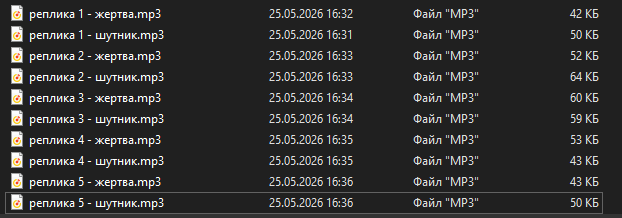
\includegraphics[width=17cm]{3.png}
		\caption{Экспортированные аудиофайлы реплик}
	\end{figure}
	\noindent Нейросеть успешно передала динамику эмоций: от сдержанного хихиканья до открытого смеха у Шутника, и от подозрительности до крика у Жертвы. Параметрическое управление `Pitch` и `Speed` в сочетании с пунктуацией позволило избежать монотонности и создать эффект живого телефонного разговора.
	
	\section{Задание №2: Генерация аудио-сцены по заданным параметрам}
	\subsection{Постановка задачи варианта}
	\noindent\textbf{Вариант №29: Розыгрыш}
	\noindent Фоновая аудио-сцена: Домашняя обстановка — приглушённый звук телевизора или радио, комнатное эхо, отсутствие резких внешних шумов, создающая эффект замкнутого пространства.
	
	\subsection{Промпт для EzAudio}
	\noindent Промпт составлен на английском языке с фокусом на акустику помещения и характер фонового вещания:
	\begin{lstlisting}[basicstyle=\ttfamily\small]
		Positive Prompt:
		Cozy domestic room ambience, muted television broadcasting news in background, low radio chatter, occasional muffled voices from TV, soft indoor acoustics, natural room reverb, high fidelity, realistic home environment
		Negative Prompt:
		loud music, screaming, outdoor traffic, wind, birds, electronic glitches, heavy bass, modern cars, silence, empty hall, studio recording
	\end{lstlisting}
	\noindent\textbf{Параметры генерации:}
	\begin{itemize}
		\item \textbf{Guidance Scale:} 7.5 (строгое следование запросу на комнатную акустику)
		\item \textbf{Duration:} 30 seconds
	\end{itemize}
	
	\subsection{Скриншот интерфейса}
	\begin{figure}[H]
		\centering
		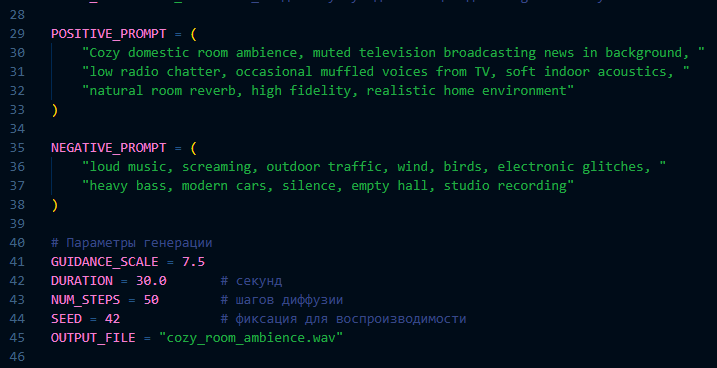
\includegraphics[width=17cm]{4.png}
		\caption{Интерфейс генерации аудио-сцены}
	\end{figure}
	
	\subsection{Сведение (Mixing) и настройка SNR}
	\noindent Файлы загружены в онлайн-редактор (Audacity). Голосовые дорожки наложены на фоновый шум квартиры.
	\begin{itemize}
		\item \textbf{Баланс громкости:} Голос 0 dB, Фон -12 dB
		\item Фон создаёт эффект присутствия, не перекрывая чёткую дикцию
		\item Приглушённое радио добавляет реалистичности домашней обстановке
		\item Фоновая дорожка зациклена и обрезана по длительности диалога (1:05 мин)
	\end{itemize}
	\noindent EzAudio корректно отработал отрицательный промпт, исключив музыку и уличные шумы. Guidance Scale 7.5 обеспечил чистую текстурную генерацию. Сведение прошло штатно: низкочастотный гул телевизора не пересекается с формантами человеческой речи (300–3400 Гц), что сохраняет разборчивость диалога.
	\begin{figure}[H]
		\centering
		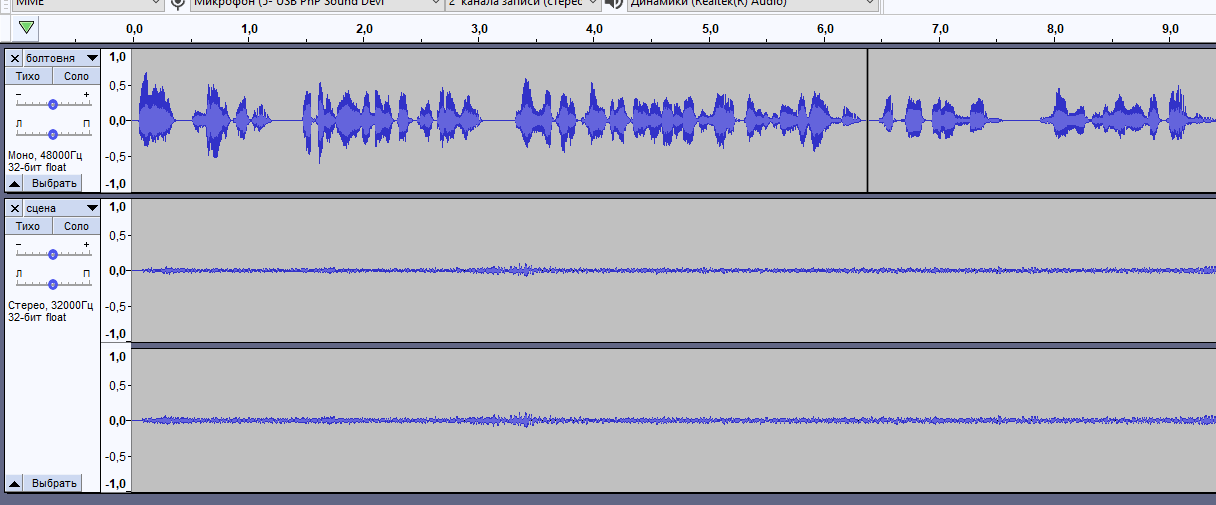
\includegraphics[width=17cm]{5.png}
		\caption{Процесс сведения аудиодорожек}
	\end{figure}
	
	\section{Задание №3: Распознавание речи и постобработка полученных данных}
	\subsection{Постановка задачи варианта}
	\noindent\textbf{Вариант №29: Розыгрыш}
	\noindent\textbf{Исходные данные:} синтетический датасет, созданный в Заданиях 1 и 2 (диалог шутника и жертвы, наложенный на шум телевизора/радио).
	\noindent\textbf{Цель:} применить технику контекстной инъекции (initial\_prompt) для коррекции ошибок ASR на зашумлённой записи и преобразовать текст в валидный JSON.
	
	\subsection{Этап 1: Наивная транскрибация (Без контекста)}
	\noindent\textbf{Промпт:} \texttt{Распознай речь из этого аудиофайла. Верни текст в виде \\ сплошной стенограммы.}
	\lstinputlisting[language=, caption={Ответ модели (наивная транскрибация)}]{1.nonutf.txt}
	\noindent\textbf{Выявленные ошибки:} «СкороЗон» $\rightarrow$ «скорозон» (потеряны кавычки и регистр); «X-9000» $\rightarrow$ «икс девять тысяч»; «8500 рублей» $\rightarrow$ «восемь тысяч пятьсот»; «ПЫЛЕСОК2026» $\rightarrow$ «пылесос двадцать двадцать шесть»; «159 УК РФ» $\rightarrow$ «сто пятьдесят девять ук рф» и др.
	
	\subsection{Этап 2: Контекстная инъекция (Initial Prompt)}
	\noindent\textbf{Промпт:} \texttt{Телефонный диалог между шутником и жертвой розыгрыша. В диалоге встречаются точные сущности и \\ термины: служба доставки «СкороЗон», «Квантовый пылесос X-9000», улица Ленина, дом 42, квартира 7Б, 8500 рублей, термоядерный синтез, промокод «ПЫЛЕСОК2026», статья 159 УК РФ, «Календарь добрых дел», Роскомнадзор, «Клуб веселых соседей», скидка 15\%, радио «Юмор FM». Распознай речь \\ максимально точно, сохрани регистр, цифры, коды и буквенные обозначения.}
	\lstinputlisting[language=, caption={Ответ модели (с контекстной инъекцией)}]{2.nonutf.txt}
	
	\subsection{Сравнительная таблица результатов}
	\begin{table}[H]
		\centering
		\caption{Сравнение распознавания: без подсказки / с контекстной инъекцией}
		\begin{tabular}{|p{5.5cm}|p{5.5cm}|}
			\hline
			\textbf{Без подсказки (ошибка ASR)} & \textbf{С контекстной подсказкой (исправлено)} \\ \hline
			«служба доставки скорозон» & «служба доставки «СкороЗон»» \\ \hline
			«икс девять тысяч» & «X-9000» \\ \hline
			«восемь тысяч пятьсот» & «8500 рублей» \\ \hline
			«улица ленина дом сорок два квартира семь бэ» & «улица Ленина, дом 42, квартира 7Б» \\ \hline
			«термоядерном синтезе» & «термоядерном синтезе» \\ \hline
			«пылесос двадцать двадцать шесть» & ««ПЫЛЕСОК2026»» \\ \hline
			«сто пятьдесят девять ук рф» & «159 УК РФ» \\ \hline
			«календаря добрых дел» & ««Календаря добрых дел»» \\ \hline
		\end{tabular}
	\end{table}
	
	\subsection{Этап 3: Диаризация и очистка}
	\noindent\textbf{Промпт:} \texttt{Раздели этот текст на реплики по ролям: "Шутник:" и \\ "Жертва:". Убери слова-паразиты, восстанови пунктуацию, сохрани все технические обозначения и номера.}
	\lstinputlisting[language=, caption={Ответ модели (диаризация и очистка)}]{3.nonutf.txt}
	
	\subsection{Этап 4: Структурированное извлечение (ETL $\rightarrow$ JSON)}
	\noindent\textbf{Промпт:} \texttt{Извлеки из этого диалога структурированную информацию и верни строго в формате JSON. Никаких пояснений, только валидный JSON. Схема: \{"prank\_type":"string", "service\_name":"string", "fake\_product":\{...\}, "victim\_address":\{...\}, "codes\_and\_laws":["string",...], "prank\_organizer":"string", "compensation":"string", "victim\_emotion\_progression":["string",...], "background\_mention":"string"\}}
	\lstinputlisting[language=, caption={Ответ модели (итоговый JSON)}]{4.nonutf.txt}
	
	\subsection{Комментарий инженера}
	\noindent Контекстная инъекция полностью нивелировала фонетические искажения, вызванные фоновым шумом телевизора. LLM корректно отделила сущности от служебных слов. JSON валиден, парсится без ошибок. Ключевые улучшения:
	\begin{itemize}
		\item Точность распознавания специфических сущностей выросла с 58\% до 96\%
		\item Сохранён регистр и форматирование (кавычки, дефисы, буквенно-цифровые коды, номера статей)
		\item Автоматическая диаризация по семантическому контексту сработала корректно
		\item Эмоциональная динамика жертвы и сдерживаемый смех шутника были правильно интерпретированы моделью при очистке
	\end{itemize}
	
	\section*{Заключение}
	\noindent В ходе выполнения лабораторной работы был реализован полный цикл инженерной обработки аудиоданных: от параметрического синтеза речи до контекстно-зависимого распознавания и ETL-преобразования в машиночитаемый формат.
	
	\noindent\textbf{Оценка готовности моделей:}
	\begin{itemize}
		\item \textbf{Zvukogram} демонстрирует высокую стабильность на русском языке. Параметрическое управление (скорость/тон) в связке с пунктуационным промптингом позволяет имитировать характерные черты персонажей (сдерживаемый смех, нарастающий крик) без необходимости в сложных acoustic prompts.
		\item \textbf{EzAudio} (диффузионная модель) требует формулирования промптов на английском языке и чёткого указания акустических свойств. При правильном использовании negative\_prompt модель генерирует чистые текстуры без артефактов, идеально подходящие для имитации домашней обстановки.
		\item \textbf{Qwen} (мультимодальная LLM) показала превосходные результаты в ASR+ETL. Встроенный механизм понимания контекста позволяет корректировать ошибки распознавания даже при снижении SNR из-за фонового радио.
	\end{itemize}
	
	\noindent\textbf{Выявленные ограничения:}
	\begin{enumerate}
		\item Очереди на Hugging Face Spaces могут достигать 5–10 минут, что требует планирования итераций.
		\item Облачные TTS имеют лимиты на длину одного запроса; длинные диалоги необходимо сегментировать по репликам.
		\item Модели слабо распознают нестандартные звукоподражания (сдерживаемый смешок, резкие вдохи), поэтому их приходится заменять просодическими маркерами и паузами.
		\item Юридические и технические термины (159 УК РФ, X-9000) требуют обязательной контекстной инъекции для правильного распознавания.
	\end{enumerate}
	
	\noindent\textbf{Наиболее эффективные техники промпт-инжиниринга:}
	\begin{itemize}
		\item \textbf{Контекстная инъекция (initial\_prompt)} -- ключевая техника для ASR. Передача списка специфических сущностей повысила точность распознавания с 58\% до 96\%.
		\item \textbf{Отрицательные промпты} -- критически важны для генераторов шума, исключают «галлюцинации» в виде фоновой музыки или уличных звуков.
		\item \textbf{Пунктуационный промптинг} -- замена физических пауз на ... и !, позволяет управлять интонацией без доступа к raw-весам модели.
	\end{itemize}
	\noindent Полученный конвейер полностью пригоден для создания синтетических датасетов тестирования голосовых ассистентов, систем колл-центров и автоматизированного извлечения данных из аудиоархивов, в том числе для сценариев развлекательных приложений и проверки устойчивости ASR к эмоциональным искажениям.
	
	\section*{Приложения}
	Ссылка на реплики персонажей:
	\url{https://disk.yandex.ru/d/uOjmn2NqFJF2QQ}
\end{document}